\documentclass{beamer}

\usepackage{amssymb,amsmath}
\usepackage{graphicx}
\usepackage{url}
\usepackage{color}
\usepackage{relsize}		% For \smaller
\usepackage{url}			% For \url
\usepackage{epstopdf}	% Included EPS files automatically converted to PDF to include with pdflatex

%For MindMaps
% \usepackage{tikz}%
% \usetikzlibrary{mindmap,trees,arrows}%

%%% Color Definitions %%%%%%%%%%%%%%%%%%%%%%%%%%%%%%%%%%%%%%%%%%%%%%%%%%%%%%%%%
%\definecolor{bordercol}{RGB}{40,40,40}
%\definecolor{headercol1}{RGB}{186,215,230}
%\definecolor{headercol2}{RGB}{80,80,80}
%\definecolor{headerfontcol}{RGB}{0,0,0}
%\definecolor{boxcolor}{RGB}{186,215,230}

%%% Save space in lists. Use this after the opening of the list %%%%%%%%%%%%%%%%
%\newcommand{\compresslist}{
%	\setlength{\itemsep}{1pt}
%	\setlength{\parskip}{0pt}
%	\setlength{\parsep}{0pt}
%}

%\setbeameroption{show notes on top}

% You should run 'pdflatex' TWICE, because of TOC issues.

% Rename this file.  A common temptation for first-time slide makers
% is to name it something like ``my_talk.tex'' or
% ``john_doe_talk.tex'' or even ``discrete_math_seminar_talk.tex''.
% You really won't like any of these titles the second time you give a
% talk.  Try naming your tex file something more descriptive, like
% ``riemann_hypothesis_short_proof_talk.tex''.  Even better (in case
% you recycle 99% of a talk, but still want to change a little, and
% retain copies of each), how about
% ``riemann_hypothesis_short_proof_MIT-Colloquium.2000-01-01.tex''?

\mode<presentation>
{
  % A tip: pick a theme you like first, and THEN modify the color theme, and then add math content.
  % Warsaw is the theme selected by default in Beamer's installation sample files.

  %%%%%%%%%%%%%%%%%%%%%%%%%%%% THEME
  %\usetheme{AnnArbor}
  %\usetheme{Antibes}
  %\usetheme{Bergen}
  %\usetheme{Berkeley}		% bem bacana - menu esquerdo
  %\usetheme{Berlin}
  %\usetheme{Boadilla}
  %\usetheme{boxes}
  %\usetheme{CambridgeUS}		% bem bacana - menu superior
  %\usetheme{Copenhagen}
  %\usetheme{Darmstadt}
  %\usetheme{default}
  %\usetheme{Dresden}
  \usetheme{Frankfurt}
  %\usetheme{Goettingen}
  %\usetheme{Hannover}		% bem bacana - menu esquerdo
  %\usetheme{Ilmenau}
  %\usetheme{JuanLesPins}
  %\usetheme{Luebeck}
  %\usetheme{Madrid}		%bacana
  %\usetheme{Malmoe}
  %\usetheme{Marburg}		% bem bacana - menu direito
  %\usetheme{Montpellier}
  %\usetheme{PaloAlto}		% bem bacana - menu esquerdo
  %\usetheme{Pittsburgh}
  %\usetheme{Rochester}		%bacana
  %\usetheme{Singapore}
  %\usetheme{Szeged}
  %\usetheme{Warsaw}

  %%%%%%%%%%%%%%%%%%%%%%%%%%%% COLOR THEME
  %\usecolortheme{albatross}		% azul escuro, massa
  %\usecolortheme{beetle}		% cinza, menu azul
  %\usecolortheme{crane}		% branco e amarelo, massa
  \usecolortheme{default}		% branco, azul clarinho
  %\usecolortheme{dolphin}		% azul e branco, legal
  %\usecolortheme{dove}			% cinza e branco, feio
  %\usecolortheme{fly}			% todo cinza, horrível
  %\usecolortheme{lily}			% parece o default
  %\usecolortheme{orchid}		% azul e branco, ok
  %\usecolortheme{rose}			% branco e violeta-claro, bonito
  %\usecolortheme{seagull}		% cinza, feio
  %\usecolortheme{seahorse}		% nhé, meio feio
  %\usecolortheme{sidebartab}		% Azul, branco, destaque na tab, interessante
  %\usecolortheme{structure}		% bichado
  %\usecolortheme{whale}		% Azul e branco, bem bonito

  %%%%%%%%%%%%%%%%%%%%%%%%%%%% OUTER THEME
  \useoutertheme{default}
  %\useoutertheme{infolines}
  %\useoutertheme{miniframes}
  %\useoutertheme{shadow}
  %\useoutertheme{sidebar}
  %\useoutertheme{smoothbars}
  %\useoutertheme{smoothtree}
  %\useoutertheme{split}
  %\useoutertheme{tree}

  %%%%%%%%%%%%%%%%%%%%%%%%%%%% INNER THEME
  \useinnertheme{circles}
  %\useinnertheme{default}
  %\useinnertheme{inmargin}
  %\useinnertheme{rectangles}
  %\useinnertheme{rounded}

  %%%%%%%%%%%%%%%%%%%%%%%%%%%%%%%%%%%

  \setbeamercovered{invisible} % or whatever (possibly just delete it)
  % To change behavior of \uncover from graying out to totally
  % invisible, can change \setbeamercovered to invisible instead of
  % transparent. apparently there are also 'dynamic' modes that make
  % the amount of graying depend on how long it'll take until the
  % thing is uncovered.

}


% Get rid of nav bar
\beamertemplatenavigationsymbolsempty

% Use short top
%\usepackage[headheight=12pt,footheight=12pt]{beamerthemeboxes}
%\addheadboxtemplate{\color{black}}{
%\hskip0.5cm
%\color{white}
%\insertshortauthor \ \ \ \ 
%\insertframenumber \ \ \ \ \ \ \ 
%\insertsection \ \ \ \ \ \ \ \ \ \ \ \ \ \ \ \ \  \insertsubsection
%\hskip0.5cm}
%\addheadboxtemplate{\color{black}}{
%\color{white}
%\ \ \ \ 
%\insertsection
%}
%\addheadboxtemplate{\color{black}}{
%\color{white}
%\ \ \ \ 
%\insertsubsection
%}

% Insert frame number at bottom of the page.
% \usefoottemplate{\hfil\tiny{\color{black!90}\insertframenumber}} 

\usepackage[english]{babel}
\usepackage[latin1]{inputenc}
\usepackage{subfigure}

\usepackage{times}
\usepackage[T1]{fontenc}

\usepackage{tikz}
\usetikzlibrary{arrows,shapes}
% Latex Graph Example:
% https://www.overleaf.com/5297501zrjzfm#/16716638/

% TODO: Silly Makefile

\tikzstyle{vertex}=[circle,fill=black!25,minimum size=10pt,inner sep=0pt]
\tikzstyle{blue vertex}=[circle,fill=blue!100,minimum size=10pt,inner sep=0pt]
\tikzstyle{red vertex}=[circle,fill=red!100,minimum size=10pt,inner sep=0pt]
\tikzstyle{edge} = [draw,thick,-]
\tikzstyle{red edge} = [draw, line width=5pt,-,red!50]
\tikzstyle{black edge} = [draw, line width=5pt,-,black!20]
\tikzstyle{weight} = [font=\smaller]

\title[GB21802]{GB21802 - Programming Challenges}
\subtitle[]{Week 7 - Math Problems}
\author[Claus Aranha]{Claus Aranha\\{\footnotesize caranha@cs.tsukuba.ac.jp}}
\institute{College of Information Science}
\date{2019-05-31,06-03\\{\tiny Last updated \today}}

\begin{document}

\section{Introduction}
\subsection{Title}
\begin{frame}
\maketitle
\end{frame}

% \subsection{Last Week Notes}
%
% \begin{frame}
  \frametitle{Results for the Previous Week}

  \begin{center}
    Here are the results for last week:

    \bigskip
    
    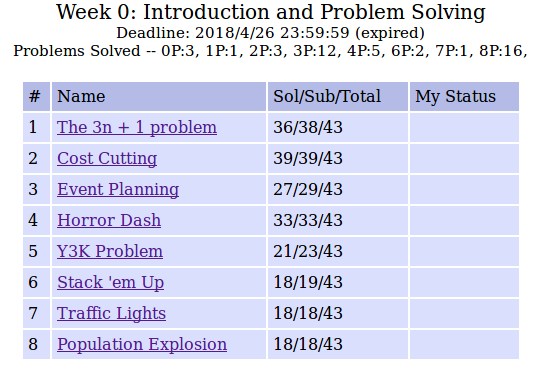
\includegraphics[width=0.8\textwidth]{img/resultW0}
    
    \bigskip

    Hope you enjoyed the warm up!
  \end{center}

\end{frame}

\begin{frame}[fragile]
  \frametitle{Comments from e-mails and questions -- 1}

  \begin{block}{Submission with Java}
    Two students had \structure{``runtime error''} with Java last week
    -- don't forget that your start class MUST be called {\bf Main}.
  \end{block}

  \vfill

\begin{verbatim}
class Main {
  public static void main(String[] args) {

    // do something...

  }
}
\end{verbatim}
\end{frame}

\begin{frame}
  \frametitle{Comments from e-mails and questions -- 2}
  \begin{block}{Input/Output}
    Two other students had problems because their program printed ``Please enter a number''.

    \bigskip

    You are very kind, but please {\bf follow the specifications} strictly!
  \end{block}
  
  \vfill

  \begin{block}{Format for MANABA submission}
    One student asked if the code for MANABA had to be the same as the code for UVA.

    \bigskip

    Yes. The code you submit on MANABA must be {\bf exactly the same}
    as the code you submitted for UVA.
  \end{block}
\end{frame}

\begin{frame}
  \frametitle{Short comments about the problems:}
  \begin{itemize}
  \item Cost Cutting, Event Planning, Horror Dash -- Easiest problems (find mean, find min, find min);
    \bigskip

  \item 3n+1 -- Still easy, but a few traps -- example of {\bf Memoization};
    \bigskip

  \item Y3K Problem -- Still easy, but skip year can be a bit troublesome.
    
  \end{itemize}
\end{frame}

%\begin{frame}
%  \frametitle{Comments about the problems}
%\end{frame}


\subsection{Outline}
\begin{frame}
  \frametitle{Outline: Math Problems}

  \begin{itemize}
    \item Math problems in programming competition normally require:
    \begin{itemize}
      \item Simple problem descriptions;
      \item A lot of time thinking;
      \item Not so much time programming;
    \end{itemize}
  \end{itemize}
\end{frame}

\begin{frame}
  \frametitle{Outline: Math Problems}

  Many math problems are {\bf ad hoc}. In this lecture we will study:
  \begin{itemize}
    \item Common Implementation Issues in Math problems: Bignum, precision, etc.
    \item Number Theory Algorithms: Factorization, Primality Testing, GCD;
    \item Combinatory Tricks: Common Sequences, Probability;
  \end{itemize}
\end{frame}


\section{Implementation Tricks}

\begin{frame}
  \frametitle{Implementation Tricks}
  \begin{itemize}
    \item BigNums;
    \item Modulo Operations;
    % \item Precision;
  \end{itemize}
\end{frame}

\subsection{Bignum}
\begin{frame}
  \frametitle{Dealing with Big Numbers}

  Some problems (specially math problems) require using very large numbers.
  For example: $25! = 15511210043330985984000000 > 10^{26}$.\bigskip

  {\bf However}:
  \begin{itemize}
    \item \structure{Maximum C++ unsigned int}: $2^{32} < 10^{11}$
    \item \structure{Maximum C++ unsigned long long}: $2^{64} < 10^{20}$
  \end{itemize}\bigskip


  \begin{block}{}
    I usually recommend to use C++; but Java is better for
    BigNum progchal problems!
  \end{block}
\end{frame}

\begin{frame}[fragile]
  \frametitle{Bignum Example: 10925 -- Krakovia}

  {\smaller
\begin{block}{}
\begin{verbatim}
import java.util.Scanner;
import java.math.BigInteger;
class Main {
  public static void main(String[] args) {
    Scanner sc = new Scanner(System.in);
    int caseNo = 1;
    while (true) {
      int N = sc.nextInt(), F = sc.nextInt();
      if (N == 0 && F == 0) break;
      BigInteger sum = BigInteger.ZERO;     // Bignum Constant
      for (int i = 0; i < N; i++) {
        BigInteger V = sc.nextBigInteger(); // Bignum I/O
        sum = sum.add(V); }
      System.out.println("Bill #" + (caseNo++)
        + " costs " + sum + ": each friend should pay "
        + sum.divide(BigInteger.valueOf(F)) + "\n" );}
  }
}
\end{verbatim}
  \end{block}}
\end{frame}


\begin{frame}[fragile]
  \frametitle{More functions from Java.math.BigInteger}
{\smaller

  \begin{block}{Algebraic functions}
    BigInteger.add(), .subtract(), .multiply(), .divide(),
    .pow(), .mod(), .remainder()
  \end{block}

  \begin{block}{Changing Number Base}
\begin{verbatim}
BI = BigInteger(10); System.println(BI.toString(2))
// Result: 1010
\end{verbatim}
  \end{block}

  \begin{block}{Probabilistic Primality Test}
\begin{verbatim}
isPrime = BI.isProbablePrime(int certainty)
// Chance of being correct is 1 - (1/2)^certainty
\end{verbatim}
  \end{block}


\begin{block}{Other cool functions}
  BigInteger.gcd(BI)
  BigInteger.modPow(BI exponent, BI m)
\end{block}}
\end{frame}

\subsection{Modulo Operations}
\begin{frame}
  \frametitle{Modulo Operation}

  {\smaller
  We can use \structure{modulo arithmetic} to operate on very large
  numbers without calculating the entire number.

  \bigskip

  Remember that:
  \begin{enumerate}
  \item $(a+b)\%s = ((a\%s)+(b\%s)+s)\%s$
  \item $(a*b)\%s = ((a\%s)*(b\%s))\%s$
  \item $(a^n)\%s = ((a^{n/2}\%s)*(a^{n/2}\%s)*(a^{n\%2}\%s))\%s$
  \end{enumerate}

  }
\end{frame}

\begin{frame}
  \frametitle{Modulo Operation -- UVA 10176, Ocean Deep!}
  {\smaller
  \begin{block}{Problem summary}
    Test if a binary number $n$ (up to 100000 digits) is divisible by 131071
  \end{block}

  \begin{itemize}
  \item The problem wants to know if $n\%13107 == 0$
  \item But $n$ is too big!

  \item Use the recurrence in the previous slide to break down each
    digit to a reasonable value.
  \end{itemize}}

\end{frame}

% \subsection{Precision}
% TODO: printing with precision in C, Java, Python
% Dealing with very small numbers

\section{Number Theory}
\subsection{outline}
\begin{frame}
  \frametitle{Number Theory} {\small

    Number Theory studies \structure{the integer numbers} and
    \structure{sets}.

    \bigskip

    \begin{itemize}
    \item Primality;
    \item Division and Remainders;
    \item Sequences of numbers;
    \end{itemize}

    }
\end{frame}

\subsection{Prime Numbers}
\begin{frame}
  \frametitle{Number Theory: Primality Testing}

  {\smaller
    \structure{Prime Numbers}: Only divisible by 1 and itself:

    \medskip

    2,3,5,7,11,13...

    \bigskip

    How do you test if a number $N$ is prime?

  \begin{itemize}

  \item Full search: For each $f \in 2..N-1$, test if $N\%f == 0$\\
    $O(N)$

    \bigskip

  \item A little Pruning: For each $f \in 2..\text{floor}(\sqrt{N})$,
    test if $N\%f == 0$\\
    $O(\sqrt(N))$

  \item Can you do it in $O(\sqrt{n} / \log(n))$?
  \end{itemize}}
\end{frame}

\begin{frame}
  \frametitle{Number Theory: Primality Testing}

  \begin{block}{The Prime Number Theorem (simplified)}
    The probability of $i < N$ is prime is $1 / \log(N)$
  \end{block}

  \hfill

  {\small

  {\bf collorary\footnote{``Collorary'' means ``consequence''} 1}: There are $N/\log(N)$ primes $<N$\\
  {\bf collorary 2}: We just need to test the {\bf primes} between 1 and $\sqrt{N}$

  \hfill

  But how do we find all primes between 1 and $\sqrt{N}$ fast?
  }
\end{frame}



\begin{frame}[fragile]
  \frametitle{Sieve of Eratosthenes}

  {\smaller
    \begin{block}{Idea}
      \begin{itemize}
      \item Start with a set from 2 to $\sqrt{N}$.
      \item Test if each $i$ in the set is prime.
      \item If $i$ is prime, remove all multiples $mi$.
      \end{itemize}
    \end{block}

  \begin{exampleblock}{}
\begin{verbatim}
def sieve(k):                 ## Find all primes up to k
   primes = []
   sieve = [1]*(k+1)    ## all numbers start in the list
   sieve[0] = sieve[1] = 0             ## except 0 and 1
   for i in range(k+1):                          ## O(N)
      if (sieve[i] == 1):
         primes.append(i)             ## new prime found
         j = i*i   ## why can i start from i*i, not i*2?
         while (j < k+1):                  ## O(loglogN)
            sieve[j] = 0
            j += i                      ## next multiple
   return primes
\end{verbatim}
  \end{exampleblock}
  }
\end{frame}

\begin{frame}
  \frametitle{Sieve of Eratosthenes}

  {\smaller
    \begin{block}{Amortized Complexity}
      \begin{itemize}
      \item The complexity of the Sieve is $O(N\log\log N)$

        \medskip

      \item If we do the Sieve every time we test for primes, we are not saving much.

        \medskip

      \item But we can do the Sieve one time, and test many primes later!

      \end{itemize}
    \end{block}

    \hfill

    When we do an expensive operation once, we call it {\bf amortized complexity}
  }
\end{frame}

% Prime number: Sosuu
% Prime factors: Soinsuu
% Factorization: Insuu Bunkai
\begin{frame}
  \frametitle{Finding Prime Factors}

  {\smaller

    Any natural number $N$ can be expressed as a \structure{unique}
    set of prime numbers:

    \begin{equation*}
      N=1p_1^{e_1}p_2^{e_2}\ldots p_n^{e_n}
    \end{equation*}

    These are the \structure{Prime Factors} of $N$. From this set, we
    can also obtain the set of \structure{Factors} of $N$ (all numbers
    $i$ where $i|N$).

    \medskip

    Factorization is a key issue in \structure{cryptography}

    \begin{block}{Very Naive approach -- Test all numbers!}
      For every $i \in 1..N/2$, test $i|N$ and isPrime(i).\\
      \smallskip
      \hfill Very Expensive!
    \end{block}

    \begin{block}{Naive approach -- Test all primes}
      Calculate a list of primes $i$ up to N/2, test if $i|N$.\\
      \smallskip
      \hfill Wrong Answer, why?
    \end{block}
}
\end{frame}

\begin{frame}[fragile]
  \frametitle{Prime factorization: Divide and conquer approach}

  {\smaller
  \begin{block}{Recursive Idea}
    The prime factorization of $N$ is equal to the union of $p_i$ and
    the prime factorization of $N/p_i$, where $p_i$ is the smallest
    prime factor of $N$.

    \bigskip

    The set of all factors is composed of all combinations of the set
    of prime factors (including repetitions).
  \end{block}

  \begin{exampleblock}{}
\begin{verbatim}
def primefactors(n):
   primes = sieve(int(np.sqrt(n))+1)
   c = 0, i = n, factors = []
   while i > 1:
      if (i%primes[c] == 0):
          i = i/primes[c]
          factors.append(primes[c])
      else:
          c = c+1
   return factors
\end{verbatim}
  \end{exampleblock}}
\end{frame}


\begin{frame}
  \frametitle{Working with Prime Factors: 10139 -- Factovisors}

  {\smaller
    \begin{block}{Problem description}
      Calculate whether $m$ divides $n!$ ($1 \leq m,n \leq 2^{31}-1$)
    \end{block}

    Factorial of 22 is already bigint! But we can break down these numbers into their
    factors, which are all $\leq 2^{30}$.

    \begin{itemize}
    \item $F_m$: primefactors(m)
    \item $F_{n!}$: $\cup$(primefactors(1), primefactors(2)...,primefactors(n))
    \end{itemize}

    Having the factor sets, $m$ divides $n!$ if $F_m \subset F_{n!}$.

    \bigskip

    Examples:
    \begin{itemize}
    \item $m = 48$ and $n=6$\\
      $F_m = \{2,2,2,2,3\} F_{n!} = \{2,3,2,2,5,2,3\}$

  \medskip

    \item $m = 25$ and $n = 6$\\
      $F_m = \{5,5\} F_{n!} = \{2,3,2,2,5,2,3\}$

    \end{itemize}
  }
\end{frame}


% Saidaikōyakusū
\subsection{GCD/LCM}
\begin{frame}[fragile]
  \frametitle{Euclid Algorithm and Extended Euclid Algorithm}

  {\smaller
    \begin{itemize}
    \item \structure{Euclid Algorithm} gives us the greatest common divisor $D$ of $a,b$;
    \item \structure{Extended Euclid Algorithm} also gives us $x,y$ so that $ax+by = D$;
    \item Both are extremely simple to code:
    \end{itemize}

    \vfill

    \begin{exampleblock}{}
\begin{verbatim}
int gcd(int a, int b) {return (a == 0?b:gcd(b%a,a));}

int x, y;
int egcd(int a, int b) {
   if (a==0)
      {x = 0; y = 1; return b;}        // stop condition
   int d = egcd(b%a, a);
   int tx = x;                         // gcd recurrence
   x = y - (b/a)*tx; y = tx; return d; }   // update x,y
\end{verbatim}
    \end{exampleblock}
}
\end{frame}

\begin{frame}
  \frametitle{Using EGCD: The Diophantine Equation}
  {\smaller
    \begin{block}{Problem Example (variations of this problem are common)}
      You have 839 yen. \alert{X}hoco candy costs 25 yen,
      \alert{Y}anilla candy costs 18 yen. How many candies can we buy?
    \end{block}

    \bigskip

    The equation $xA+yB=C$ is called the \structure{Linear Diophantine
      Equation}. It has infinite solutions if GCD(A,B)|C, but none if
    it does not.

    \bigskip

    The first solution ($x_0,y_0$) can be derived from the extended
    GCD, and other solutons can be found from:
    expressed as:
    \begin{itemize}
    \item $x = x_0 + (b/d)n$
    \item $y = y_0 - (a/d)n$
    \end{itemize}
    Where $d$ is GCD(A,B) and $n$ is an integer.
  }
\end{frame}

\begin{frame}
  \frametitle{Using EGCD: The Diophantine Equation}
  {\smaller
    \begin{block}{Problem Example (variations of this problem are common)}
      You have 839 yen. \alert{X}hoco candy costs 25 yen,
      \alert{Y}anilla candy costs 18 yen. How many candies can we buy?
    \end{block}

    \begin{itemize}
    \item \structure{EGCD} gives us: $x=-5, y=7, d=1$ or $25(-5)+18(7) = 1$
    \item Multiply both sides by 839: $25(-4195)+18(5873) = 839$
    \item So: $x_n = -4195 + 18n$ and $y_n = 5873 - 25n$
    \item We have to find $n$ so that both $x_n,y_n$ are $> 0$.
    \item $-4195 + 18n \geq 0$ and $5873 - 25n \geq 0$
    \item $n \geq 4195/18$ and $5873/25 \geq n$
    \item $4195/18 \leq n \leq 5873/25$
    \item $233.05 \leq n \leq 234.92$
    \end{itemize}
  }
\end{frame}


\section{Combinatorics}
\subsection{Counting and Closed Forms}
\begin{frame}
  \frametitle{Combinatorics problems}

  {\smaller
    \begin{block}{Definition}
      Combinatorics is the branch of mathematics concerning the study of
      \structure{countable discrete structures}.
    \end{block}

    Combinatory problems involve understanding a sequence, and
    figuring one of:

    \medskip

    \begin{itemize}
    \item \structure{Recurrence}: A formula that calculates the
      $n^{th}$ member of a sequence, based on the value of previous members;

    \item \structure{Closed form}: A formula that calculates the
      $n^{th}$ member of a sequence independently from other members;
    \end{itemize}

  \bigskip

  It is not uncommon to use \structure{Dynamic Programming} or
  \structure{Bignum} to solve combinatoric related problems.
  }
\end{frame}

\begin{frame}
  \frametitle{Example: Triangular Numbers}
  {\smaller
  \begin{block}{Definition}
    The triangular numbers is the sequence where the $n^{th}$ value is
    composed of the sum of all integers from $1$ to $n$
  \end{block}

  \begin{itemize}
  \item S(1) = 1
  \item S(2) = 1+2 = 3
  \item S(3) = 1+2+3 = 6
  \item $\ldots$
  \item S(7) = 1+2+3+4+5+6+7 = 28
  \end{itemize}
  }

  What are the recurrence and the closed form for this sequence?
\end{frame}

\begin{frame}
  \frametitle{Example: Triangular Numbers}
  {\smaller
    \begin{itemize}
    \item S(1) = 1, S(2) = 3, S(3) = 6
    \end{itemize}

    \begin{block}{Recurrence}
      The recursive form of a sequence:
      \begin{equation*}
        S(n) = S(n-1)+n; S(1) = 1
      \end{equation*}
    \end{block}
    \begin{block}{Closed Form}
      The non-recursive form of a sequence:
      \begin{equation*}
        S(n) = \frac{n(n+1)}{2}
      \end{equation*}
    \end{block}
    \alert{Problem:} Calculate the first triangle number with more
    than 500 factors!  }
\end{frame}

\subsection{Fibonacci}

\begin{frame}
  \frametitle{A more famous sequence: Fibonacci Numbers}

  {\smaller
  \begin{block}{Definition -- very famous sequence}
    Each number is the sum of the two numbers before it.

    \medskip

    F() = 0,1,1,2,3,5,8,13,21,34...
  \end{block}

  \begin{block}{The recurrence is well known}
  \begin{equation*}
  F(0) = 0, F(1) = 1, F(n) = F(n-1)+F(n-2)
  \end{equation*}
  When implementing the recurrence, don't forget the memoization
  table!
  \end{block}

  \begin{block}{Closed Form}
    The Fibonacci numbers also have a less well known
    \structure{closed form}:

    \begin{equation*}
      F(n) = \frac{1}{\sqrt{5}}\left(\left(\frac{1+\sqrt{5}}{2}\right)^n-\left(\frac{1-\sqrt{5}}{2}\right)^n\right)
    \end{equation*}
  \end{block}
    Square roots introduce floating point errors. What is the maximum
    $n$ this can calculate with less than 0.1 error?
  }
\end{frame}

\begin{frame}[fragile]
  \frametitle{Fibonacci Facts}
  {\smaller
  \begin{block}{Zeckendorf's theorem}
    Every positive integer can be written in a \structure{unique way} as a sum of
    one or more distinct fibonacci numbers, which are not consecutive.

\begin{verbatim}
def zeckenfy(n):
    fibs = []
    f = greatest fib =< n; fibs.append(f)
    fibs.append(zeckenfy(n-f))
    return fibs
\end{verbatim}
  \end{block}

  \begin{block}{Pisano's period}
    The last digits of the Fibonacci sequence repeat!

    \medskip

    The last one/two/\alert{three/four} digits repeat with a period of
    60/300/\alert{1500/15000}.

    F(6) = 8\\
    F(66) = 27777890035288\\
    F(366) = 1380356705549181797202918793682511 3333650564850089197542855968899086435571688

  \end{block}
  }
\end{frame}

\subsection{Binom}

\begin{frame}[fragile]
  \frametitle{Binomial Coefficients}
  {\smaller

    \begin{block}{Definition}
      Binomial Coefficients are the number series that correspond to
      the coefficients of the expansion of a binomial:

      \medskip

      Binom(3) = $(a+b)^3$ = $1a^3 + 3ab^2 + 3ab^2 + b^3$ = $\{1,3,3,1\}$

      \medskip

      We are usually interested in the $k^{th}$ coefficient of the
      $n^{th}$ binomial:

      \medskip

      $C(n,k) = C(3,2) = \{1,$ \alert{3} $,3,1\} = 3$

    \end{block}

    Pascal's Triangle gives us a good representation of C(n,n):
\begin{verbatim}
0  1  0  0  0  0  0  0  0  0
0  1  1  0  0  0  0  0  0  0
0  1  2  1  0  0  0  0  0  0
0  1  3  3  1  0  0  0  0  0
0  1  4  6  4  1  0  0  0  0
0  1  5  10 10 5  1  0  0  0
0  1  6  15 20 15 6  1  0  0
0  1  7  21 35 35 21 7  1  0
0  1  8  28 56 70 56 28 8  1
\end{verbatim}
  }
\end{frame}

\begin{frame}
  \frametitle{Uses for the Binomial Coefficient}

  The value of $C(n,k)$ tells us how many ways we can choose $n$
  items, $k$ at a time.

  \bigskip

  Some use cases:
  \begin{itemize}
  \item \structure{Probabilities:} What is the probability of winning
    a loto when you choose 5 numbers out of 60? $1/C(60,5)$
  \item \structure{Grids:} How many ways are there to go from the
    bottom left end of a $mn$ grid to the top right, if you can only
    go up and right? $C(m+n,n)$
  \end{itemize}
\end{frame}


\begin{frame}
  \frametitle{Calculating the Binomial Coefficient}
  {\smaller

    \begin{block}{Closed form of C(n,k)}
      \begin{equation*}
        C(n,k) = \frac{n!}{(n-k)!k!}
      \end{equation*}

      \alert{Problem}: Multiplying factorials tends to generate huge numbers
      even for small $n$ and $k$.
    \end{block}

    \begin{block}{Recurrence for C(n,k)}
      \begin{itemize}
      \item C(n,0) = C(n,n) = 1;
      \item C(n,k) = C(n-1,k-1) + C(n-1,k)
      \end{itemize}

      Using a memoization table will cut the calculation time by
      half. In this case, top-down DP will usually be faster than
      bottom-up.
    \end{block}
  }
\end{frame}

\subsection{Catalan}

\begin{frame}
  \frametitle{Another useful sequence: Catalan Numbers}
  {\smaller
  \begin{block}{The Catalan sequence}
    \begin{equation*}
      C(n) = 1, 1, 2, 5, 14, 42, 132, 429, 1430
    \end{equation*}
  \end{block}

  \begin{exampleblock}{The Recurrence}
    \begin{equation*}
    C(n) = \sum^{n-1}_{k=0}C(k)C(n-1-k)
    \end{equation*}
  \end{exampleblock}

  \begin{exampleblock}{Closed Form}
    \begin{equation*}
      C(n) = \frac{1}{n+1}\binom{2n}{n}
    \end{equation*}
  \end{exampleblock}
  }
\end{frame}

\begin{frame}
  \frametitle{Catalan Numbers -- Uses}
  \begin{itemize}
    \item Number of ways that you can match $n$ parenthesis.\\
      C(3):((())),()(()),(())(),()()(),(()())

      \medskip

    \item Number of ways that you can triangulate a poligon with $n+2$ sides
    \item Number of monotonic paths on an $nxn$ grid that do not pass above
      the diagonal.
    \item Number of distinct binary trees with $n$ vertices
    \item Etc...
  \end{itemize}
\end{frame}

\subsection{Integer Partition}
\begin{frame}
  \frametitle{Integer Partition}
  \begin{block}{}
    f(5,5) = (5),(4,1),(3,2),(3,1,1),(2,2,1),(2,1,1,1),(1,1,1,1,1)
  \end{block}
  \begin{block}{Definition and calculation}
    $f(n,k)$ -- number of ways that we can sum $n$, using integers
    equal or less than $k$.

    \bigskip

    \structure{Recurrence:}
    \begin{itemize}
    \item $f(n,k) = f(n-k,k) + f(n, k+1)$
    \item $f(1,1) = 1$; $f(n,k) = 0$ if $k > n$
    \end{itemize}
  \end{block}
\end{frame}

\begin{frame}
  \frametitle{Ad Hoc Example: Probability problems}

  {\smaller
    \begin{block}{Dice Throwing}
      If you have $n$ dice, what is the chance of rolling a total above $m$?
    \end{block}

    \begin{itemize}
    \item \structure{Example:} For $n=3$, $m=16$, what is the probability?
    \end{itemize}
  }
\end{frame}

\begin{frame}
  \frametitle{Ad Hoc Example: Probability problems}

  {\smaller
    \begin{block}{Dice Throwing}
      If you have $n$ dice, what is the chance of rolling a total above $m$?
    \end{block}

    \begin{itemize}
    \item \structure{Example:} For $n=3$, $m=16$, the chance is $10/216$

      \bigskip

    \item All combinations of 3 dice: $6*6*6 = 216$
    \item Combinations above 16:
    \end{itemize}

    \begin{columns}[T]
      \column{0.3\textwidth}
      \begin{itemize}
      \item 6,6,6
      \item 6,6,5
      \item 6,5,6
      \item 5,6,6
      \end{itemize}
      \column{0.3\textwidth}
      \begin{itemize}
      \item 6,5,5
      \item 5,6,5
      \item 5,5,6
      \end{itemize}
      \column{0.3\textwidth}
      \begin{itemize}
      \item 4,6,6
      \item 6,4,6
      \item 6,6,4
      \end{itemize}
    \end{columns}

    \medskip

    \begin{itemize}
    \item What algorithm do you use?
    \end{itemize}
  }
\end{frame}

\begin{frame}
  \frametitle{Ad Hoc example: Probabilty Problems}

  {\smaller
  \begin{block}{The dice problem}
    If I have $n$ dice, what is the chance of rolling a total above $m$?
  \end{block}

  \medskip

  Solving with DP

  \medskip

  \begin{itemize}
  \item For $n=0$, we have only one result: $r=0$
  \item For $n=1$, we have 6 results: $r = \{1,2,3,4,5,6\}$
  \item The result for $n=i$ and $r_{n-1}=k$ is $r_n = k + \{1,2,3,4,5,6\}$

    \bigskip

  \item With a state table (dice,result), we can count the number of
    dice combination above a certain value;

  \end{itemize}
  }
\end{frame}

\begin{frame}[fragile]
  \frametitle{Ad Hoc example: Probability Problems}
  \begin{exampleblock}{Example Code}
{\small
\begin{verbatim}
int count(int dice_left, int score_left) {
   if (score_left < 1) return pow(6,dice);
   if (dice_left == 0) return 0;
   if (result[dice_left][score_left] != -1)
      return result[dice_left][score_left];
   int sum = 0;
   for (int i = 0; i < 6; i++)
      sum += count(dice_left-1, score_left-(i+1))
   result[dice_left][score_left] = sum;
   return sum;
}

prob = count(n,m)/6**n;

\end{verbatim}
}
  \end{exampleblock}
\end{frame}

% TODO: Hare and tortoise algorith,

% TODO expand this, add more sequences
% TODO add a section on HOW to derive closed forms (from maths for CS class)


\subsection{Conclusion}
\begin{frame}
  \frametitle{Class Summary}
  \begin{itemize}
  \item Math Problems
  \item Java's Big Integer class
  \item Primality
  \item Modulo arithmetic
  \item GCD and Diophantine Equations
  \item Combinatorics
  \end{itemize}

  \begin{block}{}
    Next week: Geometry problems!
  \end{block}
\end{frame}

% \begin{frame}
  \frametitle{This Week's Problems}
  \begin{itemize}
  \item Dominator
  \item Forwarding Emails
  \item Ordering
  \item Place the Guards
  \item Doves and Bombs
  \item Come and Go
  \item ACM Contest and Blackout
  \item Ancient Messages
  \end{itemize}
\end{frame}

\begin{frame}
  \frametitle{Problem Hints (0)}

  {\smaller
  \begin{block}{Library!}
    For many of these problems, you will use a lot of repeated code:
    \begin{itemize}
    \item Visited Node arrays;
    \item Adjacent lists;
    \item Parent nodes;
    \end{itemize}

    \bigskip

    Prepare a template for the most common codes you use, and
    copy-paste it whenever necessary!
  \end{block}
  \begin{block}{Tricky Cases}
    \begin{itemize}
    \item Graphs with 1 or 0 Vertex
    \item Unconnected Graphs
    \item Self Loops
    \item Double edges
    \end{itemize}
  \end{block}
  }
\end{frame}

\begin{frame}
  \frametitle{Problem Hints (1)}  
  {\smaller
    \begin{block}{Dominator}
      \begin{itemize}
        \item If All paths from 0 to node B pass through node A, then node A {\bf dominates} node B;
        \item For all pair of nodes $i,j$, output ``Y'' if $i$ {\bf dominates} $j$, or ``N'' if not;
      \end{itemize}
    \end{block}

    \bigskip

    The idea of this problem is one of ``reachability'' -- can I reach
    node $j$ if I remove node $i$ from the graph?

    \bigskip

    Note: if $j$ is not connected to ``0'', then \emph{no one dominates j}
  }
\end{frame}

\begin{frame}
  \frametitle{Problem Hints (2)}
  {\smaller
    \begin{block}{Forwarding Emails}
      Every person $i$ sends e-mail only to person $j$.
      
      \bigskip
      
      What is the longest email chain?
      
      \bigskip
      
      Where does it start?
    \end{block}
    
    \begin{itemize}
    \item How do you deal with loops?
    \item Time limit is not very large, Try to find an O(n) solution!
    \end{itemize} 
  }
\end{frame}

\begin{frame}
  \frametitle{Problem Hints (3)}
  {\smaller
    \begin{block}{Ordering}
      Print all possible Orderings of a Direct Acyclic Graph

      \bigskip

      Generalize the DAG ordering algorithm which we discussed in class.
    \end{block}
    
    \begin{block}{Palace Guards}
      \begin{itemize}
        \item How do you represent the roads and junctions as a Graph?
        \item Find a ``guard-no guard'' assignment to vertices of the
          graph.
        \item First test if a solution is possible!
      \end{itemize}
    \end{block}    
  }
\end{frame}

\begin{frame}
  \frametitle{Problem Hints (4)}
  {\smaller
    \begin{block}{Doves and Bombs}
      This problem is about finding ``critical vertices'' in a
      graph. But how do you calculate the ``pigeon value'' of a
      vertex?
    \end{block}

    \begin{block}{Come and Go}
      Straight implementation of ``Strong Connected Components''. Be
      careful with tricky graphs!
    \end{block}    
  }
\end{frame}

\begin{frame}
  \frametitle{Problem Hints (5)}
  {\smaller
    \begin{block}{ACM Contest and Blackout}
      Goal: Find the {\bf First} minimum spanning Tree and the {\bf
        Second} minimum spanning Tree
    \end{block}

    \bigskip
    
    \begin{itemize}
    \item In this class we discussed how to find the Minimum Spanning Tree      
    \item How would we find the {\bf second minimum?}
    \item Idea: Maybe if we remove some edges from the graph?
    \end{itemize}
  }
\end{frame}

\begin{frame}
  \frametitle{Problem Hints (6)}
  \begin{block}{Ancient Message -- Challenge problem!}
    Count the symbols inside an image -- order does not matter!

    \bigskip

    What is the {\bf Main} difference between the symbols?
  \end{block}
    
  \begin{itemize}
  \item The shape and size of the symbols is actually not important!
  \item Before you begin programming, discover what is the real
    difference between the symbols.
  \item Hint: The numbers ``1'', ``0'', ``8'' have the same difference.
  \end{itemize}    
\end{frame}

%
% \begin{frame}
%   \frametitle{To Learn More}
%
%   Euler Project: Mathematical questions using computers:
%
%   \url{http://projecteuler.net}
% \end{frame}

\end{document}
